\documentclass[13pt,letterpaper]{article}
\usepackage{graphicx} % Required for inserting images
\usepackage{amsmath}
\usepackage{amssymb}
\usepackage{amsfonts}
\usepackage{array}
\usepackage{tikz}
\usepackage{csquotes}

\title{Discrete Math}
\author{andriel vinicius}
\date{\today}

\begin{document}

\maketitle
\tableofcontents
\section{Introdução}
\par
Diferente das outras ciências, na matemática não é a \emph{experiência} que prova seus fatos, mas sim a \textbf{lógica e dedução}.
Uma teoria é apresentada por meio de \emph{provas/demonstrações}, e a validação se dá a partir da aceitação de outros matemáticos. Cabe a nós, portanto, se perguntar: o que danado a matemática estuda?
\par
A resposta a essa pergunta pode ser intrigante: \textit{a matemática estuda os elementos \textbf{abstratos} da natureza}. Que objetos matemáticos são esses? Qualquer coisa; não importa com o que se esteja trabalhando na vida real, quando traduzido para o campo da matemática, todos os elementos se tornam ideias e o seu estudo e análise se dá por meio do \emph{raciocínio lógico}.
\par
Devido à abstração ao mundo das ideias, exige-se, na matemática, uma linguagem \emph{formal} e focada na \emph{lógica} na escrita de suas proposições, visto que, para que algo seja provado, sua justificativa tem de ser bem elaborada e que faça sentido lógico! Veja alguns casos abaixo:
\subsection{Exemplo A}
Tome a equação $\frac{2}{b} = \frac{2}{7} $ como verdadeira. Podemos simplesmente falar que $ b = 7 $ pois os numeradores são iguais? \emph{Não}! Para chegar nessa conclusão, devemos partir da equação modelo $ \frac{a}{b} = \frac{a}{c} $; elas só podem ser iguais se $a = 0$ \emph{ou} $b = c$. Voltando ao problema real, dado que $ a \ne 0 $, então, se $\frac{2}{b} = \frac{2}{7}$ é verdadeiro, então $b = 7$!
\subsection{Exemplo B}
Tome a equação $ \frac{x-1}{x} = \frac{x - 1}{ x + 1} $ como verdade. Perceba que, como no caso anterior, a equação só é verdade se $x - 1 = 0$ \emph{ou} $x = x + 1$. Note, contudo, que a segunda condição é um \emph{absurdo}, pois $x$ não é igual a $x + 1$. Portanto, temos a primeira condição a analisar:
\begin{math}
x - 1 = 0
\mapsto x = 0 + 1
\mapsto x = 1
\end{math}
Assim, está provado que "por a + b" que $ x = 1 $!
\par
Essas operações que acabamos de fazer são denominadas \textbf{demonstrações}. É por meio dessa comunicação que as ideias do matemático são registradas e passadas adiante. Elas são feitas seguindo os princípios da \emph{lógica matemática}.

\subsection{Lógica matemática}
Oriunda da filosofia clássica - lógica essa que trata das formas do pensamento em geral de modo a determinar o que é verdadeiro ou falso -, foi desenvolvida principalmente a partir do século XIX a partir da contribuição de \emph{filósofos} e \emph{matemáticos}.
\par
Para a lógica matemática foi criada uma espécie de \textbf{língua própria} para expressar as ideias dessa lógica, de modo a \emph{uniformizar} a escrita das operações lógicas e suprimir eventuais paradoxos e imprecisões linguísticas.
\subsubsection{Sistema axiomático}
Sistema no qual toda a lógica matemática foi desenvolvida, baseada primariamente nos chamados \textbf{axiomas}, afirmações aceitas como um ponto de partida que têm como fim chegar em um ponto específico.
\par
Esse sistema foi proposto por um matemático de nome "Hilbert" em 1900, que propôs que criassem um sistema axiomático do qual \emph{toda matemática poderia derivar}.
\par
Tal desafio resultou em contribuições fundamentais para áreas específicas da matemática, especialmente na \emph{Álgebra} e na \emph{Teoria dos Conjuntos}, essa que teve muita contribuição do grande Georg \textbf{Cantor}.
\par
Contudo, provou-se que, se um sistema axiomático for rico o suficiente para construir a matemática, ele:
\begin{enumerate}
    \item não será \textbf{completo}, pois há verdades que não podem ser provadas;
    \item não pode provar que não tem contradições em si mesmo.
\end{enumerate}
\par
Mas o que se tem hoje em dia? Bem, os matemáticos utilizam o sistema axiomático denominado \emph{ZFC}, que não vou adentrar aqui pois não nos interessa, é apenas a título de curiosidade.

\subsection{Matemática Discreta}
"Tá, mas onde você quis chegar com toda essa introdução e contextualização? Cadê a matemática discreta?". Bem, aqui estamos: a matemática discreta é uma área da matemática que trata acerca das \textbf{estruturas matemáticas que são finitas e/ou podem ser enumeradas}; um bom exemplo disso são os números naturais. Ela apresenta métodos de resolução diversos e utiliza constantemente do \emph{raciocínio matemático}.

\section{Lógica}

A \emph{lógica matemática} tem como base a \textbf{veracidade de uma proposição}, de modo a determinar se uma afirmação matemática é verdadeira ou falsa; às afirmações verdadeiras damos o nome de \textbf{teoremas}. Por exemplo, você provavelmente sabe que "a razão entre o perímetro e o diâmetro de uma circunferência é sempre $\pi$'". 
Isso é uma verdade inquestionável, independente do tamanho da circunferência. Note que o objeto matemático \textbf{circunferência} é \emph{diferente} do desenho da circunferência, pois, como sabemos, \emph{os objetos matemáticos são abstratos}, não existem na materialidade e são perfeitos.
\par
Na matemática, como comentado anteriormente, exige-se um grande rigor na escrita: não são admitidas como verdadeiras proposições como \emph{"Estude todos os dias", "Ela é linda",} entre outras, pois há lacunas que não foram preenchidas (quem é ela?, o que é ser "linda"?, estudar o quê?).
\subsection{Exemplo}
Mas e quanto à frase \emph{"Todo número inteiro par, maior ou igual a 4, é resultado da soma de dois números primos"}, ela é uma proposição? Sim, visto que, por definição, uma proposição é \emph{uma sentença que é considerada verdadeira ou falsa} (tem um propósito bem objetivo). Mas e quanto ao seu valor lógico, a proposição é verdadeira ou falsa? Podemos analisar, mas façamos as seguintes perguntas:
\begin{itemize}
    \item "O que é um número inteiro?"
    \item "O que é um número par?"
    \item "O que é um número?"
    \item "O que é uma soma?"
    \item ...
\end{itemize}
Note que, só neste exemplo, é possível encontrar mais camadas e camadas de perguntas, mas não é o objetivo desvendar tais questões agora. Admitemos as seguintes definições como verdades:
\begin{enumerate}
    \item \textbf{Definição 1}: \emph{Sendo $a$ e $b$ inteiros, dizemos que $a$ divide $b$ se existir um número $x$ de tal modo que $ a \times x = b $.} Assim, escrevemos $a|b$ indicando que $a$ divide $b$.
    \begin{enumerate}
    \item "6 divide 12?". Com base na definição 1, existe um número $x$ tal que $6 \times x = 12$. Tomemos, portanto, $x = 2$. Agora me diz: 0 é divisor de algum número inteiro? Para isso, suponha, por absurdo, que deve existir um número $z$ tal que $ 0 \times z = b$; no entanto, por definição, o produto de 0 com qualquer número resulta no próprio 0. Então, 0 é divisor de um número inteiro, mas somente dele e de nenhum outro número.
    \item Podemos tirar algumas conclusões dessa definição, como:
    \begin{itemize}
        \item -5 é divisor de 100: $(-5) \times (-20) = 100$;
        \item 21 é divisor de -441: $21 \times (-21) = (-441)$;
        \item 1 e -1 são divisores de quaisquer inteiros: $(-1) \times x = b$.
    \end{itemize}
    \end{enumerate}
    
    \item \textbf{Definição 2}: um número $a$ é par se $2|a$, ou seja, se existe um inteiro $b$ tal que $a = 2 \times b$.
    \begin{itemize}
        \item \emph{Tentativa de} Prova: suponha, por negação, que $a$ não é par, de modo que $ a \ne 2 \times b$ (2 não divide $a$). Porém, por definição, $2|a$, o que nos leva a uma contradição. Se a negação da proposição nos leva a uma contradição, a proposição por si só é verdadeira.
        \footnote{Talvez isso aqui contenha um erro, vou verificar depois.}
    \end{itemize}
    \item \textbf{Definição 3}: um inteiro $a$ é ímpar se existe um inteiro $k$ tal que $a = (2 \times k) + 1$.
    \item \textbf{Definição 4}: um inteiro $p$ é primo se, e somente se, $ p > 1 $ e os únicos divisores de $p$ forem 1 e $p$.
\end{enumerate}

Com base nessas definições, vamos analisar as seguintes proposições e, depois, verificar se a proposição inicial \emph{"Todo número inteiro par, maior ou igual a 4, é resultado da soma de dois números primos"} é verdadeira.

\begin{enumerate}
    \item \emph{"A soma de dois inteiros pares é par"}: com base na Definição 1, tomemos dois inteiros $a$ e $b$, tais que, sendo $x$ e $y$ inteiros quaisquer, $2 \times x = a$ e $2 \times y = b$. Se a soma deles é par, então existe um inteiro $n$ tal que $a + b = 2 \times n$. Como $a = 2 \times x$ e $b = 2 \times y$, temos:
    \begin{equation}
        a + b = 2 \times n
        \Longrightarrow (2 \times x) + (2 \times y) = 2 \times n
        \Longrightarrow 2 \times (x + y) = 2 \times n
    \end{equation}
    Podemos concluir, portanto, que $x + y = n$, e que a proposição inicial é verdadeira e ela é um teorema! 
    \item \emph{"Se o produto dos inteiros $a$ e $b$ for par, um dos dois inteiros é par"}: suponha que os dois inteiros são ímpares, ou seja, tal situação nos deixa com os inteiros $a = (2 \times k) + 1$ e $b = (2 \times j) + 1$, onde $k, j$ são inteiros quaisquer.
    Sendo $n$ o produto $a \times b$, a expressão originada a partir da proposição será, portanto:
        \begin{align*}
        a \times b = n &\implies 
        ((2 \times k) + 1) \times ((2 \times j) + 1) = a \times b \\ &\implies 
        4kj + 2k + 2j + 1 = a \times b \\ &\implies
        2 \times (2kj + k + j) + 1 = a \times b \\ &\implies
        2 \times c + 1 = a \times b
        \end{align*}
    Reduzindo a expressão ao inteiro $c$, temos que o produto $a \times b$ é ímpar, o que é uma contradição, já que no ínício definimos tal produto como par! Então, a contraposição da proposição é falsa, o que torna a proposição verdade!
    \footnote{Acredito que a demonstração não está errada não, mesmo sendo eu quem fiz; de qualquer forma, a proposição é mesmo verdadeira.}
    \item \emph{"Se $a|b$ e $b|a$, então $a = b$"}: essa proposição é falsa, vejamos um contraexemplo. Sejam os inteiros $a = 1$ e $b = -1$; temos que $ 1 \times (-1) = (-1)$ e $(-1) \times (-1) = 1$. No entanto, $a \ne b$!
    \item \emph{"Todo número inteiro par, maior ou igual a 4, é resultado da soma de dois números primos"}: essa afirmação é uma \textbf{Conjectura}; não se sabe de nenhum contraexemplo até o presente momento, mas também é algo que não se pode provar de maneira abstrata pelas proposições acima nem outras.
\end{enumerate}
Pode ter sido muita informação por agora, mas isso é algo que a gente se acostuma com o tempo. De toda forma, vamos dar uma olhada na "linguagem da lógica", que nos permitiu fazer todas essas operações.

\section{Linguagem e Lógica}
Como notado e utilizado, a linguagem matemática deve ser muito precisa e todos os seus termos, declarados. A partir daqui, devemos observar com mais aprofundamento os aspectos da linguagem matemática, mais precisamente como sua lógica é construída.
\subsection{Princípios básicos da proposição}
Uma proposição deve obedecer às seguintes restrições:
\begin{enumerate}
    \item \textbf{Princípio da identidade}: uma proposição verdadeira é verdadeira, e uma falsa é falsa;
    \item \textbf{Princípio da não-contradição}: nenhuma proposição pode ser verdadeira e falsa simultaneamente; 
    \item \textbf{Princípio do terceiro excluído}: uma proposição só pode ser verdadeira \textbf{ou} falsa, não havendo uma terceira possibilidade.
\end{enumerate}
Por mais que pareça algo óbvio, é fundamental que tais princípios sejam definidos antes de proposições serem operadas para evitar contradições e sabermos as "regras" do jogo.
\subsection{Tabela-verdade e Conjunções}
Na lógica, a estrutura da \emph{tabela-verdade} serve para listar todos as possibilidades de uma interação entre proposições. Tomando as proposições A e B, é possível listar seus valores da seguinte forma: \\
\begin{align*}
\begin{tabular}{c|c}
A & B \\
\hline
V & V \\
V & F \\
F & V \\
F & F \\
\end{tabular}
\end{align*}

Agora, temos o total de possibilidades da interação entre as proposições. No entanto, elas ainda não estão se relacionando; para que isso aconteça, devemos utilizar das \emph{conjunções}, de modo a manipular esses valores e gerar um valor final. Vamos analisar cada uma das conjunções:

\subsubsection{Conjunção \emph{AND}}
A conjunção \emph{and}, escrita como $\land$, gera somente um valor verdadeiro \emph{se as duas proposições forem verdadeiras}.
Tabela-verdade:
\begin{align*}
    \begin{tabular}{cc|c}
         A & B & A $\land$ B  \\
        \hline
         V & V & V \\
         V & F & F \\
         F & V & F \\
         F & F & F \\
    \end{tabular}
\end{align*}

\subsubsection{Conjunção \emph{OR}}
A conjunção \emph{or}, escrita como $\lor$, gera um valor verdadeiro quando \emph{ao menos uma proposição é verdadeira}.
Tabela-verdade:
\begin{align*}
    \begin{tabular}{cc|c}
         A & B & A $\lor$ B \\
         \hline
         V & V & V \\
         V & F & V \\
         F & V & V \\
         F & F & F \\
    \end{tabular}
\end{align*}

\subsubsection{Conjunção \emph{XOR}}
A conjunção \emph{xor}, escrita como $\vee$, gera um valor verdadeiro quando \emph{uma proposição é verdadeira ou outra}.
Tabela-verdade:
\begin{align*}
    \begin{tabular}{cc|c}
         A & B & A $\vee$ B \\
         \hline
         V & V & F \\
         V & F & V \\
         F & V & V \\
         F & F & F \\
    \end{tabular}
\end{align*}

\subsubsection{Conjunção \emph{IMPLIES}}
A conjunção \emph{implies}, escrita como $\implies$, indica as relações:
\begin{itemize}
    \item \emph{Se A, então B};
    \item \emph{A somente, se B};
    \item \emph{A é condição suficiente para B};
    \item \emph{B segue de A};
    \item \emph{B é condição necessária para A}.
\end{itemize}
Ou seja, ela gera um valor positivo em todos os casos exceto quando a proposição $B$ for falsa, pois $B$ é consequência de $A$. 
\textbf{OBS.:}: Se $A \implies B$, então $\lnot B \implies \lnot A$.
Tabela-verdade:
\begin{align*}
    \begin{tabular}{cc|c}
         A & B & A $\implies$ B  \\
         \hline
         V & V & V \\
         V & F & F \\
         F & V & V \\
         F & F & V \\
    \end{tabular}
\end{align*}

\subsubsection{Conjunção \emph{IF AND ONLY IF}}
A conjunção de equivalência \emph{if and only if}, escrita como $\iff$, indica a relação \emph{"A se, e somente se B"} e \emph{"A é condição necessária e suficiente para B"}, de modo que gera um valor positivo somente quando as duas têm o mesmo valor.
Tabela-verdade:
\begin{align*}
    \begin{tabular}{cc|c}
         A & B & A $\iff$ B  \\
         \hline
         V & V & V \\
         V & F & F \\
         F & V & F \\
         F & F & V \\
    \end{tabular}
\end{align*}

\subsubsection{Conjunção \emph{NOT}}
Ao contrário das anteriores, a conjunção \emph{not}, escrita como $\lnot$, \textbf{inverte o valor de uma proposição}. Ou seja, a tabela-verdade seria:
\begin{align*}
    \begin{tabular}{c|c}
        A & $\lnot$ A  \\
        \hline
        V & F \\
        F & V \\
    \end{tabular}
\end{align*}

\subsection{Prova e Demonstração}
Uma demonstração consiste em uma argumentação, de forma irrefutável, de que uma proposição é verdadeira. Se a proposição puder ser demonstrada, ela é denominada \emph{Teorema}; antes de ser provada, a proposição é denominada \emph{conjectura}.
Existem algumas formas de demonstração, como:
\subsubsection{Demonstração direta $A \implies B$}
Este tipo de demonstração consiste em utilizar argumentos convincentes para justificar que, se $A$ (\emph{Hipótese}) é verdadeira, $B$ (\emph{Tese}), por consequência, também é.  
Sua estrutura consiste em:
\begin{enumerate}
    \item Suponha que a hipótese ($A$) é verdadeira;
    \item Utilize de argumentos lógicos convincentes para chegar em $B$;
    \item Conclua, por fim, que a tese ($B$) é verdadeira;
\end{enumerate}
Analisemos o seguinte caso: \emph{"Sejam $a, b, c \in \mathbb{Z}$. Se $a|b$ e $b|c$, então $a|c$"}.
\begin{itemize}
    \item Hipótese: "Suponha que $a, b, c \in \mathbb{Z}$, de modo que $a|b$ e $b|c$."
    \item Tese: "Concluímos, portanto, que $a|c$." \footnote{Há um erro bastante comum nessa demonstração que é \emph{pressupor que a tese é verdadeira} e acabar usando-a durante a prova, algo que é incorreto, pois a tese é onde queremos chegar e não sabemos se ela é verdadeira ou não!} 
    \item Rascunho: Se $a|b$, então existe um inteiro $x$ de modo que $a \times x = b$, da mesma forma que se $b|c$, existe um inteiro $y$ de modo que $b \times y = c$. Como a tese diz que $a|c$, então existe um inteiro $z$ de modo que $a \times z = c$.
    Assim, teremos a seguinte situação:
    \begin{align*}
    c &\implies 
    b \times y \\ &\implies
    (a \times x) \times y \\
    \end{align*}
    Como $a \times z = c$, e $z = x \times y$, está provado que $a|c$. Vamos à demonstração de fato:
    \item \textbf{Prova}: Suponha $a, b, c \in \mathbb{Z}$, tal que $a|b$ e $b|c$. Ou seja, existem $x, y \in \mathbb{Z}$
    tal que $a \times x = b$ e $b \times y = c$. Seja também $z = x \times y$. Assim, teremos: 
    \begin{align*}
        a \times z \\ &\implies
        a \times (x \times y) \\ &\implies
        (a \times x) \times y \\ &\implies
        b \times y \\ &\implies
        c
    \end{align*}
    Logo, existe um inteiro $z$ tal que $a \times z = c$.
\end{itemize}

\subsubsection{Demonstração por Contraposição}
A demonstração por contraposição consiste em uma subversão da demonstração direta $A \implies B$. Como dito na seção acerca da conjunção \emph{implies}, se $A \implies B$, logo $\lnot B \implies \lnot A$ - lembrando que a negação de uma proposição altera o seu valor (verdadeiro $\rightarrow$ falso e vice-versa).
Sua estrutura é:
\begin{enumerate}
    \item Suponha $\lnot B$;
    \item Elabore e utilize argumentos convincentes para chegar a $\lnot A$;
    \item Conclua $\lnot A$.
\end{enumerate}
Analisemos o seguinte caso: \emph{"Sejam $a, b, n$ inteiros positivos. Se $n = a \times b$, então $ a \leq \sqrt{n}$ ou $b \leq \sqrt{n}$"}.
\begin{itemize}
    \item Não-Tese: Suponha, por contraposição, que $a \leq \sqrt{n}$ ou $b \leq \sqrt{n}$ é falso.
    \item Não-Hipótese: Então, $n = a \times b$ é falso.
    \item \textbf{Prova}: Considere que sabemos todas as propriedades das raízes quadradas e não precisamos definí-las aqui. Se $a$ e $b$ não satisfazem às condições da tese, então a não-tese é verdadeira e concluímos que $a > \sqrt{n}$ ou $b > \sqrt{n}$. Analisando a primeira desigualdade $a > \sqrt{n}$, podemos multiplicar ambos os lados por $b$:
    \begin{align*}
        a \times b > \sqrt{n} \times b
    \end{align*}
    Com a segunda desigualdade $b > \sqrt{n}$, podemos multiplicar ambos os lados por $\sqrt{n}$:
    \begin{align*}
        \sqrt{n} \times b > \sqrt{n} \times \sqrt{n} &\implies
        \sqrt{n} \times b > n
    \end{align*}
    Unindo as duas desigualdades, temos:
    \begin{align*}
        a \times b > \sqrt{n} \times b > n
    \end{align*}
   Como $a \times b > n$, não podemos ter $a \times b = n$, portanto.
    
\end{itemize}

\subsubsection{Demonstração $A \iff B$}
A demonstração \emph{se e somente se} se dá do mesmo modo da demonstração direta com um detalhe a mais: devemos provar $A \implies B$ e $B \implies A$; nessa demonstração, o resultado será verdadeiro se ambas as proposições forem verdadeiras ou falsas.
Analisemos o seguinte caso: \emph{"Um inteiro $a$ é par se, e somente se, $a + 1$ é ímpar."}
\begin{itemize}
    \item Hipótese: $a$ é um inteiro e é par;
    \item Tese: $a + 1$ é um inteiro e ímpar;
    \item \textbf{Prova}: Seja $a$ um inteiro par. Provemos primeiro que $a$ é par e $a + 1$ é ímpar. Se $a$ é par, existe um inteiro $x$ tal que $a = 2 \times x$; se $a + 1$ é ímpar, existe $a + 1 = 2 \times x + 1$ e, portanto, $a + 1$ é ímpar.
    Por fim, provemos que $a + 1$ é ímpar e $a$ é par.
    Se $a + 1$ é ímpar, existe um inteiro $x$ tal que $a + 1 = 2 \times x + 1$; subtraindo -1 de ambos os lados da equação, temos $a = 2 \times x$. Se $2|a$, $a$ é par.
    
\end{itemize}

\subsubsection{Demonstração por Contradição}
A demonstração por contradição consiste em provar que uma proposição é verdadeira negando-a e chegando em um absurdo, ou seja, em uma situação impossível. Assim, se a negação da proposição é impossível, a proposição é obrigatoriamente verdadeira. \footnote{Curiosamente, alguns teoremas matemáticos são provados exatamente desse jeito, o que evidencia o seu caráter objetivo.}
Analisemos o seguinte caso: \emph{"A soma de dois números ímpares $x$ e $y$ é sempre um número par."}
\begin{itemize}
    \item Sejam $x, y \in \mathbb{Z}$, tais que existem $m, n \in \mathbb{Z}$ de modo que $x = 2 \times m + 1$ e $y = 2 \times n + 1$, ou seja, $x$ e $y$ são ímpares. Seja também $a$ um inteiro par, ou seja, existe um inteiro $b$ tal que $a = 2 \times b$. Suponha que $x + y \ne a$ e analisemos:
    \begin{align*}
        x + y \ne a &\implies
        (2 \times m + 1) + (2 \times n + 1) \ne 2 \times b \\ &\implies
        2 \times (m + n + 1) \ne 2 \times b \\
    \end{align*}
    Perceba que ambos os lados da desigualdade são múltiplos de 2, portanto, pares, gerando uma contradição com $x + y = a$. Assim, a proposição inicial é verdadeira. \footnote{Devo verificar se isso está totalmente coerente.}
\end{itemize}

\section{Introdução à teoria dos Conjuntos}
A definição de \emph{conjunto} é algo abstrato, que não é necessariamente preciso muitas vezes; portanto, para este estudo, diremos que \emph{um conjunto é definido somente por seus elementos}. A partir disso podemos fazer a pergunta: "dado um conjunto $A$ e um elemento $x$, $x$ pertence a $A$?"
\par
Conforme visto na parte de lógica, uma proposição só pode assumir um valor verdadeiro ou falso; logo, o elemento $x$ pertence ou não pertence a $A$, ou seja, se for verdadeiro, $x \in A$, caso contrário, $x \notin A$. Contudo, devemos definir e entender as relações que existem neste tópico de conjuntos.

\subsection{Pertinência}
\subsubsection{Definição de Pertinência}
\textbf{Definição 1}: tomando um objeto $x$ e um conjunto $A$, dizemos que \emph{$x$ pertence a $A$} se $x$ for um elemento de $A$ e o denotamos como $x \in A$.
Também dizemos que \emph{$x$ não pertence a $A$} se $x$ não for um elemento do conjunto $A$ e o denotamos como $x \notin A$.
\par
\textbf{Exemplo}: Seja o conjunto $P$ = \{$x$; $x$ é primo\}. Assim, temos algumas relações existentes nesse conjunto, como: 
\begin{enumerate}
    \item $17 \in P$;
    \item $4 \notin P$;
    \item $1 \notin P$.
    \item ...
\end{enumerate}
Ampliando o escopo da relação, temos que dois conjuntos $A$ e $B$ são \emph{iguais} se necessariamente eles têm os mesmos elementos; dessa forma, eles serão diferentes somente quando existir $y$ tal que $y \in A$ e $y \notin B$ ou vice-versa.
\par
Além disso, a definição de conjunto não impede que um elemento $x$ de um conjunto $X$ seja um conjunto $Z$. Por exemplo, seja $Q$ = \{\{$4, 3, 7$\}, $2$, $3$\}:
\begin{itemize}
    \item $\{$4, 3, 7$\} \in Q$;
    \item $2 \in Q$;
    \item $7 \notin Q$.
\end{itemize}
Note que, desse modo, a nomenclatura de "elemento" e "conjunto" é variável e depende da relação do elemento com o conjunto: o elemento 7 pertence ao conjunto $\{4, 3, 7\}$ (este que é elemento de $Q$), mas não pertence ao conjunto $Q$.
\subsubsection{Conjunto Vazio}
\textbf{Definição 2}: o conjunto $A$ que não possui elementos $x$ é denominado \emph{conjunto vazio} e denotado por $\emptyset$. Perceba que ele pode ser entendido a princípio como um conjunto $A$ tal que $A = \{x; x \notin A\}$, mas isso é, na verdade, um \emph{paradoxo}, então não consideremos essa definição.

\subsection{Inclusão}
\subsubsection{Definição de Inclusão}
\textbf{Definição 3}: tomados dois conjuntos $A$ e $B$, dizemos que $A$ \emph{está contido em} $B$ se, e somente se, todos os elementos $x \in A$ também $x \in B$, da mesma forma que dizemos que $B$ \emph{está contido em} $A$ se, e somente se, todos os elementos $y \in B$ também $y \in A$. Utilizando símbolos, dizemos, no primeiro caso, que $A \subseteq B$ e, no segundo, $B \subseteq A$. Para indicar que um conjunto $A$ não está contido em $B$, utilizamos $ A \nsubseteq B$. \\
\textbf{Exemplo}: Sejam $T$ o conjunto de todos os triângulos em um plano e $P$ o conjunto de polígonos de um plano. Como um triângulo é um polígono, sabemos logo que $T \subseteq P$. No entanto, nem todo polígono é um triângulo: tomando um quadrado $q$ de lados iguais, temos que $q \in P$, mas $q \notin T$. Logo, $P \nsubseteq T$. \\
\textbf{Proposição de Inclusão Universal do $\emptyset$}: \emph{Para todo conjunto $A$, vale $\emptyset \subseteq A$}.
\begin{itemize}
    \item \emph{Demonstração}: utilizando-se da demonstração por contradição, suponha que, para todo conjunto $A$, $\emptyset \nsubseteq A$, ou seja, existe um elemento $x$ tal que $x \in \emptyset$ mas $x \notin A$. Contudo, isso é um absurdo, pois um conjunto vazio não pode ter nenhum elemento. Portanto, a proposição é sempre verdadeira.
\end{itemize}
\textbf{Definição 4}: Tomados dois conjuntos $A$ e $B$, denominamos de \emph{inclusão própria} a relação quando $A \subseteq B$ mas $A \ne B$; o símbolo utilizado para indicar tal situação é: $A \subsetneq B$. \\
\subsubsection{Propriedades} 
Para quaisquer conjuntos $A, B, C$ são válidos:
\begin{enumerate}
    \item \emph{Reflexividade}: $A \subseteq A$;
    \begin{itemize}
        \item Suponha que $A \nsubseteq A$. Conforme a definição 3, então deve existir um elemento $x$ tal que $x \in A$ e $x \notin A$; obviamente, isso gera um completo absurdo. Logo, a propriedade é verdadeira.
    \end{itemize}
    \item \emph{Antissimetria}: Se $A \subseteq B$ e $B \subseteq A$, então $A = B$;
    \begin{itemize}
        \item Se tomados os elementos $x$ de $A$ um a um de forma que $x \in A$ e $x \in B$, então $A \subseteq B$. Da mesma forma, se tomados os elementos $y$ de $B$ de modo que $y \in B$ e $y \in A$, então $B \subseteq A$. Assim, se os dois conjuntos estão inclusos um no outro, então $A = B$.
    \end{itemize}
    \item \emph{Transitividade}: Se $A \subseteq B$ e $B \subseteq C$, então $A \subseteq C$.
    \begin{itemize}
        \item Seja $x \in A$. Se $A \subseteq B$, então $x \in B$. Da mesma forma, se $B \subseteq C$, $x \in C$. Assim, $A \subseteq C$.
    \end{itemize}
\end{enumerate}
\subsubsection{Outros}
\textbf{Definição 5}: dado o conjunto $A$, denominamos de \emph{Conjuntos das Partes de A} o conjunto formado por todos os subconjuntos de $A$ (incluindo o vazio e ele mesmo).

\subsection{Operações}
As operações entre conjuntos tem por objetivo manipular e gerar um conjunto novo a partir de outros já concebidos, igual ou diferente.

\subsubsection{União}
\textbf{Definição 6}: dados os conjuntos $A$e $B$, define-se a união $A \cup B$ como sendo o conjunto formado por elementos que pertencem a pelo menos $A$ ou $B$, ou seja:
\begin{displaymath}
    A \cup B = \{ x; x \in A \text{ ou } x \in B \}
\end{displaymath}

\subsubsection{Interseção}
\textbf{Definição 7}: dados os conjuntos $A$e $B$, define-se a interseção $A \cap B$ como sendo o conjunto formado por elementos que pertencem a ambos $A$ e $B$, ou seja:
\begin{displaymath}
    A \cap B = \{ x; x \in A \text{ e } x \in B \}
\end{displaymath}

\subsubsection{Propriedades da Interseção e União}
\textbf{Observação}: algumas propriedades fazem uso de um tal \emph{conjunto universo}, representado por $\mathbb{U}$, que nada mais é que o total de conjuntos possíveis em uma situação de conjuntos. Ele deve ser fixado e, a partir disso, todos os outros conjuntos estarão contidos em $\mathbb{U}$.
Sejam os conjuntos $A, B, C$ e esteja fixado $\mathbb{U}$. Temos: \footnote{Não quis fazer a demonstração aqui para não gastar muito tempo, visto que a demonstração não é algo requerido na disciplina e eu gosto de fazer somente para fins de aprendizado, e eu já as fiz anteriormente no meu caderno.}
\begin{enumerate}
    \item  
    \begin{enumerate}
        \item $A \subseteq A \cup B$;
        \item $A \cap B \subseteq A$.
    \end{enumerate}
    \item Interação com o conjunto universo
    \begin{enumerate}
        \item $A \cup \mathbb{U} = \mathbb{U}$;
        \item $A \cap \mathbb{U} = A$.
    \end{enumerate}
    \item Interação com o conjunto vazio
    \begin{enumerate}
        \item $A \cup \emptyset = A$;
        \item $A \cap \emptyset = \emptyset$.
    \end{enumerate}
    \item Comutividade
    \begin{enumerate}
        \item $A \cup B = B \cup A$;
        \item $A \cap B = B \cap A$.
    \end{enumerate}
    \item Associatividade
    \begin{enumerate}
        \item $(A \cup B) \cup C = A \cup (B \cup C)$;
        \item $(A \cap B) \cap C = A \cap (B \cap C)$.
    \end{enumerate}
    \item Distributividade
    \begin{enumerate}
        \item $A \cap (B \cup C) = (A \cap B) \cup (A \cap C)$;
        \item $A \cup (B \cap C) = (A \cup B) \cap (A \cup C)$.
    \end{enumerate}
\end{enumerate}

\subsubsection{Complementar}
\textbf{Definição 8}: dado um conjunto $A$, denominamos de \emph{complementar} o conjunto formado pelos elementos que não compõem $A$ e denotamos como:
\begin{displaymath}
    A^C = \{x; x \notin A\}.
\end{displaymath}
\textbf{Propriedades}: fixado $\mathbb{U}$, temos as seguintes propriedades para os conjuntos $A$ e $B$:
\begin{enumerate}
    \item $\mathbb{U}^C = \emptyset$ e $\emptyset^C = \mathbb{U}$;
    \item $(A^C)^C = A$;
    \item Se $A \subseteq B$, então $B^C \subseteq A^C$;
    \item Leis de De Morgan:
    \begin{enumerate}
        \item $(A \cup B)^C = A^C \cap B^C$;
        \item $(A \cap B)^C = A^C \cup B^C$
    \end{enumerate}
\end{enumerate}

\subsubsection{Diferença}
\textbf{Definição 9}: a diferença do conjunto $A$ por $B$ é o conjunto
\begin{displaymath}
    A \backslash B = \{x; x \in A \text{ e } x \notin B \}
\end{displaymath}
Note que, a partir dessa definição, concluímos que $A^C = \mathbb{U} \backslash A$. Mas perceba que não necessariamente $A \backslash B = B \backslash A$. 
\\
\textbf{Proposição}: \enquote{Os conjuntos $A \backslash B$ e $A \cap B^C$ são iguais}.
\begin{enumerate}
    \item Primeiro, provemos que $(A \backslash B) \subseteq A \cap B^C$:
    \begin{itemize}
        \item Seja $x$ um elemento arbitrário do conjunto $A \backslash B$, ou seja, $x \in A$ mas $x \notin B$. Sabendo que $B^C$ é o conjunto de todos os elementos que não estão em $B$, podemos concluir que $x \in (A \cap B^C)$, já que, como definido, $x \in A$ e $x \notin B$. Assim, está provado que $(A \backslash B) \subseteq A \cap B^C$.
    \end{itemize}
    \item Agora, provemos que $A \cap B^C \subseteq (A \backslash B)$:
    \begin{itemize}
        \item Seja $y \in A \cap B^C$, ou seja, $y \in A$ e $y \notin B$, pois $B^C$ é o conjunto de todos os elementos que não pertencem a $B$. Logo, é possível concluir que $y \in (A \backslash B)$, já que tal conjunto também tem como elementos $y \in A$ e $y \notin B$! Assim, é provado que $A \cap B^C \subseteq (A \backslash B)$.
    \end{itemize}
    \item Estando provados que cada um dos conjuntos contém o outro, eles são, na verdade, iguais, já que cada elemento de um corresponde ao mesmo elemento do outro.
\end{enumerate}
\subsection{Conjuntos e Lógica}
Aqui está uma tabela que resume as relações e operadores dos Conjuntos e sua conversão na lógica matemática:
\begin{center}
    \begin{tabular}{c|c}
        Relação em Conjunto & Fórmula de Lógica  \\
        \hline
        $A = B$ & $P \iff Q$ \\
        $A \subseteq B$ & $P \implies Q $\\
        $A^C $ & $ \lnot P$ \\
        $A \cup B$ & $P \vee Q $ \\
        $ A \cap B$ & $P \land Q $ \\
    \end{tabular}
\end{center}

\subsection{Números}
\subsubsection{Naturais}
Denominamos de \emph{números naturais} aqueles que pertencem ao conjunto:
\begin{displaymath}
    \mathbb{N} = \{0, 1, 2, ..., n, n + 1, ...\}
\end{displaymath}
\emph{Observação}: denotamos $\mathbb{N}^*$ o conjunto $\mathbb{N} \backslash \{0\}$.

\subsubsection{Inteiros}
Denominamos de \emph{números inteiros} aqueles que pertencem ao conjunto:
\begin{displaymath}
    \mathbb{Z} = \{..., -m, -m + 1, ..., 0, +1, +2, ..., +n, +n + 1, ...\}
\end{displaymath}
\emph{Observação}: a partir da operação de \enquote{diferença}, é possível gerar os conjuntos
\begin{itemize}
    \item $\mathbb{Z}^* = Z \backslash \{0\}$;
    \item $\mathbb{Z}_+ = \{ x; x \ge 0 \}$;
    \item $\mathbb{Z}^*_+ = \{ x; x > 0 \}$;
    \item $\mathbb{Z}_- = \{ x; x \leq 0 \}$;
    \item $\mathbb{Z}^*_- = \{ x; x < 0 \}$.
\end{itemize}

\subsubsection{Racionais}
Denominamos de \emph{números racionais} aqueles que pertencem ao conjunto:
\begin{displaymath}
    \mathbb{Q} = \{\frac{p}{q} ; p, q \in \mathbb{Z}, q \ne 0 \}
\end{displaymath}
A representação pode ser finita ($\frac{12}{30},...$) ou uma dízima periódica 
($0.123123...$).

\subsubsection{Irracionais}
Denominamos de \emph{números irracionais} aqueles que têm uma representação decimal infinita e não-periódica, como $\pi$ e $\sqrt{2}$. Para estes, não há um "padrão" que defina seu conjunto, chamado de $\mathbb{I}$.

\subsubsection{Reais}
Denominamos de \emph{números reais} aqueles que pertencem ao conjunto:
\begin{displaymath}
    \mathbb{R} = \mathbb{Q} \cup \mathbb{I}
\end{displaymath}
A partir do conjunto dos reais, podemos definir o conjunto dos irracionais como resultado de:
\begin{displaymath}
    \mathbb{I} = \mathbb{R} \backslash \mathbb{Q}
\end{displaymath}
\textbf{Observação}: entre dois números reais há, pelo menos, um número irracional e outro racional.

\subsection{Intervalos reais}
Sejam $a, b \in \mathbb{R}$. O intervalo \emph{aberto} entre eles é o subconjunto:
\begin{displaymath}
    ]a, b[ = \{ x \in \mathbb{R}; a < x < b\}
\end{displaymath}
Por outro lado, o intervalo \emph{aberto} é:
\begin{displaymath}
    [a, b] = \{ x \in \mathbb{R}; a \leq x \leq b\}
\end{displaymath}
Existem algumas possibilidades, como $[a, b[$, $] - \infty, b] $ e outras. \\ Note que $ ]-\infty, +\infty [ = \mathbb{R}$.

\subsection{Exercícios de Conjuntos - A TERMINAR} 
\begin{enumerate}
    \item 
        \enquote{De que outras formas podemos representar o conjunto vazio utilizando as duas notações de definição de conjuntos que conhecemos?}
        \\
        \emph{Primeira}: Seja $\emptyset = \{\}$. \\
        \emph{Segunda}: Seja $\emptyset = \{x; x \notin \mathbb{U} \}$.
    \item \enquote{Decida quais das afirmações a seguir estão corretas. Justifique suas respostas.}
    \begin{enumerate}
        \item $\emptyset \in \emptyset$;
        \begin{itemize}
            \item \textbf{Proposição falsa}: se $\emptyset \in \emptyset$, significa que $\emptyset$ tem ao menos um elemento, o que vai contra sua definição e nos leva a um absurdo.
        \end{itemize}
        \item $\emptyset \subseteq \emptyset$;
        \begin{itemize}
            \item \textbf{Proposição verdadeira}: suponha que $\emptyset \nsubseteq \emptyset$. Logo, há um elemento $x \in \emptyset$ que não pertence a $\emptyset$. Isso gera um paradoxo óbvio, além de que, por definição, o conjunto vazio não aceita elementos. Logo, a proposição é verdadeira.
        \end{itemize}
        \item $\emptyset \in \{\emptyset\}$;
        \begin{itemize}
            \item \textbf{Proposição verdadeira}: tomado o conjunto $A = \{\emptyset\}$, suponha que $\emptyset \notin \{\emptyset\}$. No entanto, sabendo que o conjunto $A$ tem $\emptyset$ como elemento, chegamos a uma contradição. Logo, a proposição é verdadeira.
        \end{itemize}
        \item $\emptyset \subseteq \{\emptyset\}$.
        \begin{itemize}
            \item \textbf{Proposição verdadeira}: tome o conjunto $A = \{\emptyset\}$. De acordo com a Inclusão Universal do $\emptyset$, para todo conjunto $A$, vale $\emptyset \subseteq A$. Desse modo, a proposição é verdadeira.
        \end{itemize}
    \end{enumerate}
    \item \enquote{Considere $A = \{ x \in \mathbb{Z}_+ ; x < 3 \}$. Calcule $\mathbb{P}(A)$.} \\
    Temos que $\mathbb{P}(A)$ é o conjunto das partes de $A$. Logo, temos $\mathbb{P}(A) = \{\emptyset, \{0\}, \{1\}, \{2\}, \{0, 1\}, \{1, 2\}, A \}$
    \item \enquote{Dê exemplos de conjuntos $A, B, C$, justificando com os cálculos, que satisfaçam:}
    \begin{enumerate}
        \item \enquote{$A \cup (B \cap C) \ne (A \cup B) \cap C$. Qual o conjunto que será sempre igual a $A \cup (B \cap C)$?}
        \begin{itemize}
            \item 
        \end{itemize}
    \end{enumerate}
\end{enumerate}

\section{Operações Básicas}
Definem-se 2 operações fundamentais na matemática a partir da teoria dos conjuntos numéricos: a \emph{adição} e \emph{multiplicação}. Delas, advém a \emph{subtração}, onde a diferença $x - y$ pode ser vista como $x + (-y)$, e a \emph{divisão}, pois a divisão de $\frac{z}{w}$ pode ser entendida também como $z \times \frac{1}{w}$.
\subsection{Potenciação}
\textbf{Definição 10}: a potência $n \in \mathbb{N}^*$ de um número real $a$ é entendida como a multiplicação do número $a$ por ele mesmo $n$ vezes, ou seja:
\begin{displaymath}
    a \times a \times a \times a \times ... = a^n
\end{displaymath}
\textbf{Definição 11} (Propriedades): Sendo $a, b, m, n \in \mathbb{R}$, temos:
\begin{enumerate}
    \item Se $a \ne 0$, então $a^0 = 1$;
    \item $a^{-n} = \frac{1}{a^n}$ e $a^{1/n} = \sqrt[n]{a}$, se $n \in \mathbb{R}^*_+$;
    \item $a^m \times a^n = a^{m+n}$;
    \item $\frac{a^m}{a^n} = a^{m-n}$;
    \item $(a^m)^n = a^{m \times n}$;
    \item $a^{m^n} = a^{m \times m \times m \times m ...}$;
    \item $(a \times b)^n = a^n \times b^n$;
    \item $(\frac{a}{b})^n = \frac{a^n}{b^n}$;
    \item $a^{\frac{m}{n}} = \sqrt[n]{a^m}$.
\end{enumerate}

\emph{Observação}: não é correto dizer, por exemplo, que $\sqrt{4} = \pm 2$, pois essa expressão não responde qual é a raiz de 4, mas sim quais os valores que, quando elevados a 2, resultam em 4 (2 e -2).  Portanto, prefira utilizar $\sqrt{4} = 2$.

\section{Equações e Inequações}
Equações e inequações são ferramentas matemáticas poderosas e básicas de encontrar valores de incógnitas que tornem uma proposição verdadeira. 

\subsection{Equação do 1º Grau}
Uma equação do primeiro grau é uma equação da forma
\begin{displaymath}
    ax + b = 0
\end{displaymath}
onde $a, b, x  \in \mathbb{R}$, de modo que $a \ne 0$ e $x$ é denominada \textbf{incógnita}.
\subsubsection{Propriedades}
Sejam $a, b, c, d \in \mathbb{R}$. Assim, valem:
\begin{enumerate}
    \item Se $a = c$ e $b = d$, então $a + c = b + d$;
    \item Se $a = b$, então $a + c = b + c$;
    \item Se $a = c$ e $b = d$, então $a \times c = b \times d$;
    \item Se $a = b$, então $a \times c = b \times c$.
\end{enumerate}
\textbf{Exemplo A}: resolva $2x + \frac{x}{5} = 121$. \\
\emph{Resolução}:
\begin{align*}
    2x + \frac{x}{5} = 121 (\times 5) &\implies 
    10x + x = 605 \\ &\implies
    11x = 605 \quad (\times \frac{1}{11}) \\ &\implies 
    x = \frac{605}{11} \\ &\implies 
    x = 55
\end{align*}
\textbf{Exemplo B}: se $x$ representa um dígito na base 10 na equação
\begin{displaymath}
    x11 + 1x1 + 11x = 777,
\end{displaymath}
qual o valor de $X$? \\
\emph{Resolução}: Seja $x \in \{0, 1, 2, ..., 9 \}$, então:
\begin{align*}
    x11 + 1x1 + 11x = 777 &\implies 
    (100x + 11) + (10x + 100 + 1) + (x + 110) = 777 \\ &\implies
    100x + 10x + x + 222 = 777 \quad (-222) \\ &\implies
    111x = 777 - 222 \\ &\implies
    111x = 555 \quad (\times \frac{1}{111}) \\ &\implies
    x = 5
\end{align*}
\emph{Para que fique mais fácil de enxergar a reescrita na primeira linha, suponha que $x = 9$, faça as operações, compare com a equação e note que o algarismo 9 sempre vai substituir o lugar do $x$}.

\subsection{Equação de várias variáveis}

\subsection{Sistema de equações lineares}

\subsection{Equação de 2º Grau}

\subsection{Inequações de 1º Grau}

\subsection{Inequações de 2º Grau}

\section{Funções}
\textbf{Definição de Função}: função é uma \emph{relação binária} $f: X \rightarrow Y$ ($f$ de $X$ em $Y$) de um conjunto $X$ (\textbf{domínio}) com um conjunto $Y$ (\textbf{contra-domínio}), onde existem $x \in X, y \in Y$ e podemos associar o objeto $x$ ao $y$ através da função $f$, de notação $f(x) = y$. \\
\textbf{Definição de Imagem}: denominamos de \textbf{Imagem} os conjuntos abaixo:
\begin{itemize}
    \item O conjunto $f(x) = \{y \in Y; \text{existe } x \in X \text{ onde } f(x) = y \} \subseteq Y$ é denominado \textbf{Imagem de f}. No exemplo a seguir, a Imagem de $f$ é $\{x, y, z \}$;
    \item Dado $x \in X$, o único elemento $y$ tal que $y = f(x) \in Y$ correspondente é chamado de \textbf{Imagem de x}. Em outras palavras, a imagem de $x$ é o elemento $y$ com o qual ele está associado. 
\end{itemize}
\subsection{Lei de Associação da Função}
Só é considerada função uma relação que obecede às seguintes regras:
\begin{enumerate}
    \item \textbf{Todo} elemento de $X$ deve estar associado a algum elemento de $Y$;
    \item Cada elemento de $X$ só pode estar associado a um \textbf{único} elemento de $Y$ (só pode ter uma imagem).
\end{enumerate}
Ou seja, a função é uma relação binária dos tipos \emph{um para um} e \emph{muitos para um}, já que estas relações permitem com que os elementos do domínio estejam relacionadas a somente 1 elemento do contra-domínio (mesmo que, no caso da \enquote{muitos para um}, um elemento do contra-domínio esteja associado a mais de 1 elemento do domínio). \\
Exemplo de função:
\begin{center}
  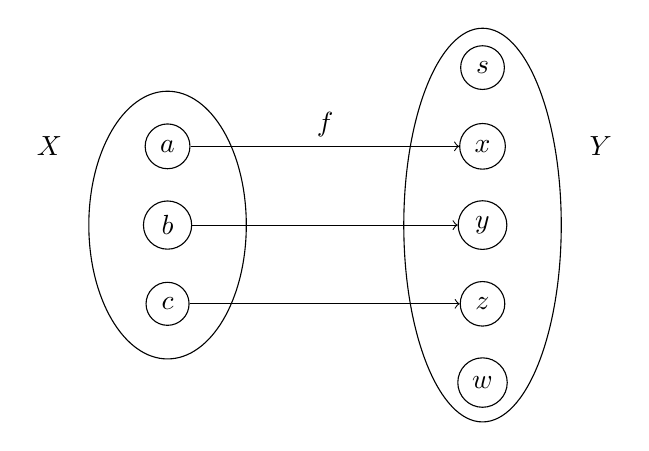
\begin{tikzpicture}
  % Conjunto X
  \draw (0, 0) ellipse (1cm and 1.7cm);
  \node at (-1.5, 1) {$X$};
  \node[circle, fill=white!30, draw] (a1) at (0, 1) {$a$};
  \node[circle, fill=white!30, draw] (a2) at (0, 0) {$b$};
  \node[circle, fill=white!30, draw] (a3) at (0, -1) {$c$};

  % Conjunto Y
  \draw (4, 0) ellipse (1cm and 2.5cm);
  \node at (5.5, 1) {$Y$};
  \node[circle, fill=white!30, draw] (b0) at (4, 2) {$s$};
  \node[circle, fill=white!30, draw] (b1) at (4, 1) {$x$};
  \node[circle, fill=white!30, draw] (b2) at (4, 0) {$y$};
  \node[circle, fill=white!30, draw] (b3) at (4, -1) {$z$};
  \node[circle, fill=white!30, draw] (b4) at (4, -2) {$w$};

  % Linhas e setas
  \draw[->] (a1) -- (b1);
  \draw[->] (a2) -- (b2);
  \draw[->] (a3) -- (b3);
  
  \node[above] at (2, 1) {$f$};
\end{tikzpicture}
\end{center}
\emph{Note que essa função obedece às regras de que todos os elementos de $X$ estão associados a um elemento de $Y$, e somente a um elemento.} \\
Mas e essa função aqui:

\begin{center}
    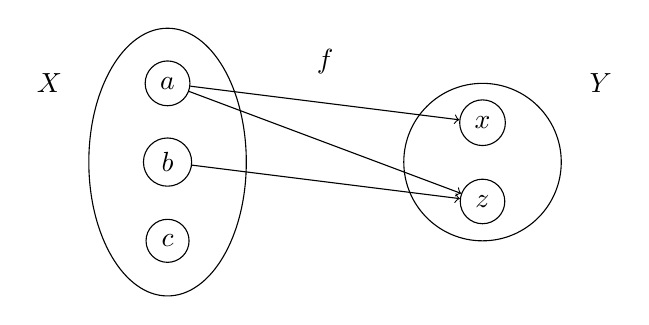
\begin{tikzpicture}
  % Conjunto X
  \draw (0, 0) ellipse (1cm and 1.7cm);
  \node at (-1.5, 1) {$X$};
  \node[circle, fill=white!30, draw] (a1) at (0, 1) {$a$};
  \node[circle, fill=white!30, draw] (a2) at (0, 0) {$b$};
  \node[circle, fill=white!30, draw] (a3) at (0, -1) {$c$};

  % Conjunto Y
  \draw (4, 0) ellipse (1cm and 1cm);
  \node at (5.5, 1) {$Y$};
  \node[circle, fill=white!30, draw] (b1) at (4, 0.5) {$x$};
  \node[circle, fill=white!30, draw] (b3) at (4, -0.5) {$z$};

  % Linhas e setas
  \draw[->] (a1) -- (b1);
  \draw[->] (a1) -- (b3);
  \draw[->] (a2) -- (b3);
  
  \node[above] at (2, 1) {$f$};
  \end{tikzpicture}
\end{center}

Ela está certa? É de fato uma função? \\
De fato isso não é uma função: primeiro, note que o elemento $c$ não está associado a nenhum elemento em $Y$; então, perceba também que $f(a) = x$ e $f(a) = z$ mas $x \ne y$, o que faz $a$ ter duas imagens, o que não é permitido. \\

\textbf{Exemplo A}: Considere as funções:
\begin{align*}
    p: \mathbb{R} \rightarrow \mathbb{R}_+ &\\ 
    x \rightarrow x^2; \\
    q: \mathbb{R}_+ \rightarrow \mathbb{R} &\\
    x \rightarrow \sqrt{x};
\end{align*} 
Qual o domínio, contra-domínio e lei de associação de cada uma das funções? \\
\emph{Resolução}:
\begin{enumerate}
    \item Função $p$:
    \begin{itemize}
        \item Domínio: \textbf{Reais};
        \item Contra-domínio: \textbf{Reais não-negativos};
        \item Lei de associação: $p(x) = x^2$.
    \end{itemize}
    \item Função $q$:
    \begin{itemize}
        \item Domínio: \textbf{Reais não-negativos};
        \item Contra-domínio: \textbf{Reais};
        \item Lei de associação: $q(x) = \sqrt{x}$.
    \end{itemize}
\end{enumerate}
\subsection{Identidade}
\textbf{Definição de Identidade}: Seja $I_x : X \rightarrow X$ tal que $I_x(x) = x$ para todo $x \in X$. Denominamos essa função de \textbf{Função Identidade}; ou seja, todo elemento do domínio aponta para ele mesmo no contra-domínio.

\subsection{Função Injetora}
\textbf{Definição de Injetividade}: denominamos de \emph{injetiva} uma função de relação binária \enquote{1 para 1}, de modo que, para todos $x_1, x_2 \in X$, $x_1 \ne x_2$ que implica que $f(x_1) \ne f(x_2)$. Em outras palavras, cada elemento da imagem de $f$ está ligado a somente um elemento de $X$. \\
\emph{Definições alternativas}: 
\begin{enumerate}
    \item $f$ é injetiva se, e somente se, para todos os $x_1, x_2 \in X$, $f(x_1) = f(x_2) \implies x_1 = x_2$;
    \item $f$ é injetiva se, para cada $y \in f(X)$ (imagem de $f$), existir somente um $x \in X$ tal que $y = f(x)$.
\end{enumerate}
Diagrama de uma função injetiva:
\begin{center}
    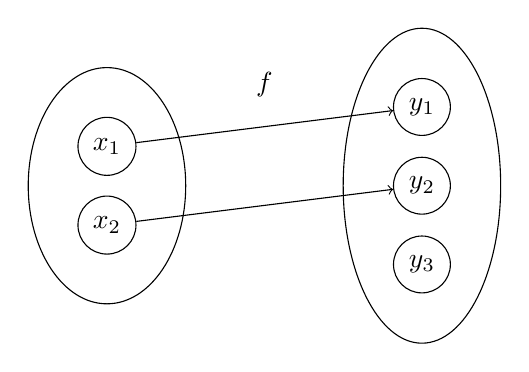
\begin{tikzpicture}
      % Conjunto X
      \draw (0, 0) ellipse (1cm and 1.5cm);
      \node[circle, draw] (x1) at (0, 0.5) {$x_1$};
      \node[circle, draw] (x2) at (0, -0.5) {$x_2$};
      % Conjunto Y
      \draw (4, 0) ellipse (1cm and 2cm);
      \node[circle, draw] (y1) at (4, 1) {$y_1$};
      \node[circle, draw] (y2) at (4, 0) {$y_2$};
      \node[circle, draw] (y3) at (4, -1) {$y_3$};
      % Função f
      \draw[->] (x1) -- (y1);
      \draw[->] (x2) -- (y2);
        \node[above] at (2, 1) {$f$};
    \end{tikzpicture}
\end{center}

\textbf{Exemplo B}: considerando as funções $p, q$ da seção \enquote{Lei de Associação das Funções}, elas são de qual classificação? \\
\emph{Resolução}:
\begin{itemize}
    \item Função $p$: \textbf{não é injetiva}. Sendo $x_1 = 2, x_2 = (-2)$, note o seguinte caso: \footnote{Para provar algo, devo partir de alguma definição. Parti, portanto, da primeira das definições alternativas.}
    \begin{align*}
        f(x_1) = f(x_2) \implies
        f(2) = f(-2) \implies
        2 = -2
    \end{align*}
    Tal conclusão é um absurdo. Logo, a função $p$ não é injetiva, já que dois elementos diferentes têm a mesma imagem.
    \item Função $q$: \textbf{é injetiva}. Sejam $x_1, x_2 \in \mathbb{R}_+$ tais que:
    \begin{align*}
        f(x_1) = f(x_2) &\implies
        \sqrt{x_1} = \sqrt{x_2} \\ &\implies
        (\sqrt{x_1})^2 = (\sqrt{x_2})^2 \\ &\implies
        x_1 = x_2
    \end{align*}
    Logo, a função $q$ é injetiva segundo a primeira definição alternativa.
\end{itemize}
\subsection{Função Sobrejetora}
\textbf{Definição de Sobrejetividade}: denominamos de \emph{sobrejetiva} uma função $f$ tal que $f(X) = Y$, ou seja, onde a imagem é equivalente ao contra-domínio. \\
\emph{Definição alternativa}: $f$ é sobrejetiva se, para todo $y \in Y$, existe $x \in X$ (não necessariamente um único $x$) tal que $f(x) = y$. \\

Diagrama de uma função sobrejetiva:

\begin{center}
    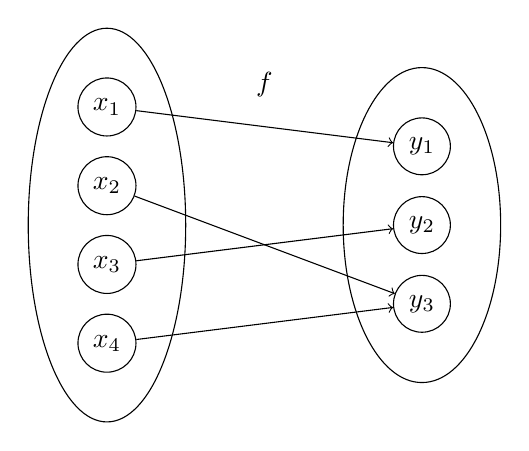
\begin{tikzpicture}
      % Conjunto X
      \draw (0, 0) ellipse (1cm and 2.5cm);
      \node[circle, draw] (x1) at (0, 1.5) {$x_1$};
      \node[circle, draw] (x2) at (0, 0.5) {$x_2$};
      \node[circle, draw] (x3) at (0, -0.5) {$x_3$};
      \node[circle, draw] (x4) at (0, -1.5) {$x_4$};
      % Conjunto Y
      \draw (4, 0) ellipse (1cm and 2cm);
      \node[circle, draw] (y1) at (4, 1) {$y_1$};
      \node[circle, draw] (y2) at (4, 0) {$y_2$};
      \node[circle, draw] (y3) at (4, -1) {$y_3$};
    
      % Função f
      \draw[->] (x1) -- (y1);
      \draw[->] (x2) -- (y3);
      \draw[->] (x3) -- (y2);
      \draw[->] (x4) -- (y3);
        \node[above] at (2, 1.5) {$f$};
      
    \end{tikzpicture}
\end{center}

\textbf{Exemplo C}: considerando as funções $p$ e $q$ das seções anteriores, elas são sobrejetivas? \\
\emph{Resolução}:
\begin{itemize}
    \item Função $p$: \textbf{é sobrejetiva}. Provemos que $Im_p = \mathbb{R_+}$. Por definição, $Im_p \subseteq \mathbb{R_+}$. Então, seja $r \in \mathbb{R_+}$, para qualquer $r$; temos que $\sqrt{r} \in \mathbb{R}$, logo, executando a função temos:
    \begin{displaymath}
        p(x) = x^2 \implies p(\sqrt{r}) = (\sqrt{r})^2 \implies p(\sqrt{r}) = r
    \end{displaymath}
    Portanto, como a operação é válida para todo $r \in \mathbb{R_+}$, temos que $\mathbb{R_+} \subseteq Im_p$. Então, $Im_p = \mathbb{R_+}$.
    
    \item Função $q$: \textbf{não é sobrejetiva}, pois não existe $x \in \mathbb{R_+}$ tal que $\sqrt{x} = -1$, e $-1 \in \mathbb{R}$ (contra-domínio) mas não pertence a $\mathbb{R_+}$ (domínio).

\end{itemize}

\subsection{Função Bijetora}
\textbf{Definição de Bijetividade}: denominamos de $bijetiva$ a função $f$ que é sobrejetiva e injetiva simultaneamente, ou seja, se, e somente se, para todo $y \in Y$, existe um $x \in X$ tal que $f(x) = y$.

Diagrama de uma função bijetora:
\begin{center}
    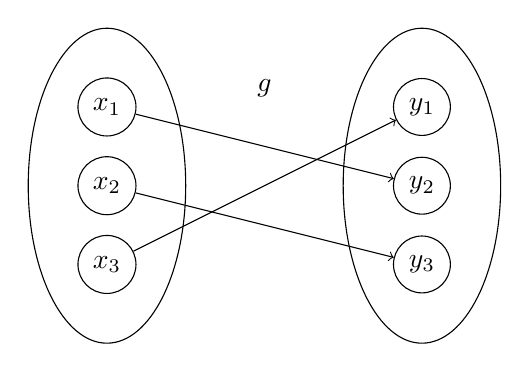
\begin{tikzpicture}
      % Conjunto X
      \draw (0, 0) ellipse (1cm and 2cm);
      \node[circle, draw] (x1) at (0, 1) {$x_1$};
      \node[circle, draw] (x2) at (0, 0) {$x_2$};
      \node[circle, draw] (x3) at (0, -1) {$x_3$};
      % Conjunto Y
      \draw (4, 0) ellipse (1cm and 2cm);
      \node[circle, draw] (y1) at (4, 1) {$y_1$};
      \node[circle, draw] (y2) at (4, 0) {$y_2$};
      \node[circle, draw] (y3) at (4, -1) {$y_3$};
    
      % Função f
      \draw[->] (x1) -- (y2);
      \draw[->] (x2) -- (y3);
      \draw[->] (x3) -- (y1);
        \node[above] at (2, 1) {$g$};
      
    \end{tikzpicture}
\end{center}
Note que, como $p$ e $q$ não são sobrejetivas e injetivas simultaneamente, elas não são bijetivas!

\subsection{Função Composta}
\textbf{Definição de Composta}: Sejam as funções 
\begin{align*}
    f: X \rightarrow Y, \\
    g: Z \rightarrow W,
\end{align*}
de modo que o domínio de $g$ é equivalente ao contra-domínio de $f$, logo $Y \subseteq Z$. Denominamos de \textbf{função composta} a função de $g$ com $f$ com domínio em $X$ e contra-domínio em $W$, denotada por $g \circ f$, e que a cada $x \in X$ satisfaz 
\begin{displaymath}
    W = (g \circ f) (x) \implies g(f(x)) \in W
\end{displaymath} \\

Diagrama de uma função composta:
\begin{center}
    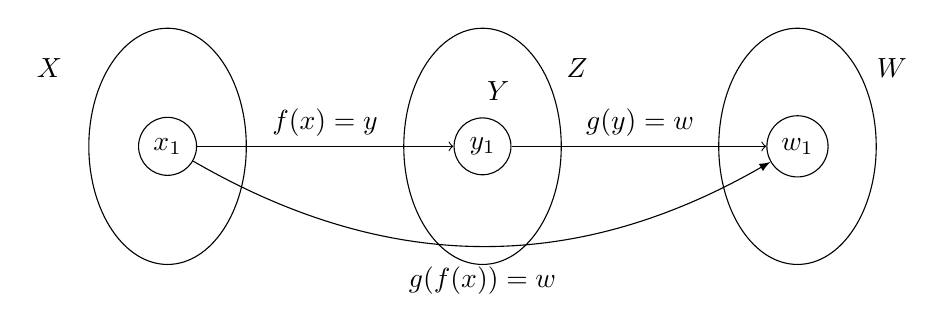
\begin{tikzpicture}
        \node at (-1.5, 1) {$X$};
      \draw (0, 0) ellipse (1cm and 1.5cm);
      \node[circle, draw] (x1) at (0, 0) {$x_1$};
      % Conjunto Z
      \node at (5.2, 1) {$Z$};
      \draw (4, 0) ellipse (1cm and 1.5cm);
      \node at (4.2, 0.7) {$Y$};
      \node[circle, draw] (y1) at (4, 0) {$y_1$};
      % Conjunto W
      \draw (8, 0) ellipse (1cm and 1.5cm);
      \node at (9.2, 1) {$W$};
      \node[circle, draw] (w1) at (8, 0) {$w_1$};
    
      % Função f
      \draw[->] (x1) -- (y1);
        \node[above] at (2, 0) {$f(x) = y$};
      \draw[->] (y1) -- (w1);
        \node[above] at (6, 0) {$g(y) = w$};
      \draw[-latex] (x1) to[bend right] (w1);
      \node [above] at (4,-2) {$g(f(x)) = w$};
    \end{tikzpicture}
\end{center}
\textbf{Exemplo A}: Sejam 
\begin{align*}
f(x) = e^x, &\\
g(x) = x^2 - 1. 
\end{align*}
Calcule $f \circ g$ e $g \circ f$.
\\
\emph{Resolução}:
\begin{enumerate}
    \item $f$ de $g$:
    \begin{align*}
        f \circ g &\implies f(g(x)) \\ &\implies
        f(x^2 - 1) \\ &\implies
        f(x^2 - 1) = e^{x^2-1}
    \end{align*}
    \item $g$ de $f$:
    \begin{align*}
        g \circ f &\implies g(f(x)) \\ &\implies
        g(e^x) = {(e^x)}^2 - 1 \\ &\implies
        g(e^x) = e^{2x} - 1
    \end{align*}
\end{enumerate}
\textbf{Exemplo B}: Sendo $f: X \rightarrow Y$, mostre que:
\begin{enumerate}
    \item $f \circ I_x = f$ \\
    \emph{Resolução}:
    O domínio de $f \circ I_x$ é $X$, pois advém da função identidade, 
    enquanto seu contra-domínio é $Y$, que advém da função $f$.
    Tomando $x \in X$ para qualquer $x$, podemos saber a lei de associação ao executar a função:
    \begin{displaymath}
        (f \circ I_X)(x) \implies f(I_x(x)) \implies f(x)
    \end{displaymath}
    Então, é possível definir a função composta da seguinte forma:
    \begin{align*}
        f \circ I_x: &\ X \rightarrow Y \\
        & x \rightarrow f(x),
    \end{align*}
    que é exatamente equivalente à função $f$.

    \item $I_y \circ f = f$ \\
    \emph{Resolução}:
    O domínio de $I_y \circ f$ é $X$, pois vem de $f$, enquanto seu contra-domínio é $Y$, o qual vem de $I_y$.
    Tomando $x \in X$ para qualquer $x$, temos:
    \begin{displaymath}
        (I_y \circ f)(x) \implies I_y(f(x)) \implies I_y(y) \implies y = f(x)
    \end{displaymath}
    Portanto, definimos a função composta assim:
    \begin{align*}
        I_y \circ f: &\ X \rightarrow Y \\
        & x \rightarrow f(x),
    \end{align*}
    exatamente igual à função $f$.
\end{enumerate}

\subsection{Função Inversa}
\textbf{Definição de Inversa}: denominamos de \emph{Função Inversa} uma função \textbf{Bijetora}\footnote{Somente funções bijetoras podem ser inversas.} $f: X \rightarrow Y$ se existe uma outra função $f^{-1}: Y \rightarrow X$\footnote{Pode receber qualquer outro nome, como $g$} tal que:
\begin{itemize}
    \item $f \circ f^{-1} = I_Y$;
    \item $f^{-1} \circ f = I_X$.
\end{itemize}
\textbf{Exemplo A}: calcule a inversa da função $f(x) = 4x - 8$. \\
\emph{Resolução passo a passo:}
\begin{enumerate}
    \item \textbf{Atribua $y = f(x)$}: $y = 4x - 8$;
    \item \textbf{Troque $x$ por $y$}: $x = 4y - 8$;
    \item \textbf{Isole o $y$}: $4y = x + 8 \implies y = \frac{x + 8}{4}$
    \item \textbf{Substitua $y$ pela inversa}: $f^{-1} = \frac{x + 8}{4}$
\end{enumerate}
\textbf{Exemplo B}: Verifique se as funções anteriormente definidas $p$ e $q$ são inversas.
\\
\emph{Resolução}: \\
Verifiquemos $q \circ p: \mathbb{R} \rightarrow \mathbb{R}$. Temos:
    \begin{align*}
        (q \circ p)(x) &\implies q(p(x)) \\
        &\implies q(x^2) \\
        &\implies \sqrt{x^2} \\
        &\implies |x|
    \end{align*}
Como $|x| \ne I_x$, temos que as funções $p$ e $q$ não são inversas.

\section{To Be Continued...}
\end{document}
